\setlength\tabcolsep{1mm}
\renewcommand\arraystretch{1.3}
\newcounter{Figura}
\renewcommand\theFigura{\arabic{Figura}}
\newcounter{Tabla}
\renewcommand\theTabla{\arabic{Tabla}}

\chapter{Análisis}
\label{capitulo2}
	
{\selectlanguage{spanish}
	A continuación se presentan los aspectos más importantes que se tuvieron en cuenta para el desarrollo del proyecto. Se
	presentan características deseadas en un sistema de intercambio de información de seguridad entre organizaciones.}

\section{Análisis de requerimientos}
{\selectlanguage{spanish}
	Existen distintos problemas que obstaculizan el intercambio de información entre las organizaciones. Dichas
	problemáticas afectan la reputación, seguridad y la capacidad de trabajo de las organizaciones. }

{\selectlanguage{spanish}
	Las organizaciones pueden intercambiar grandes volúmenes de datos los cuales pueden provenir de diferentes fuentes, cada
	una de estas fuentes puede utilizar una representación propia para los datos. Por ello es deseado que las
	organizaciones utilicen un estándar aceptado por todas. La representación utilizada debería permitir el desarrollo de
	herramientas que ayuden a la organización y estructuración de los datos de forma de facilitar el trabajo de los
	analistas.}

{\selectlanguage{spanish}
	Otro de los problemas que interfieren en el intercambio de información es el riesgo a la seguridad y reputación de la
	organización. La información intercambiada debe pasar por procesos que controlen los datos que se intercambien evitando
	de esta manera la divulgación de información sensible o privada.}

{\selectlanguage{spanish}
	Estas son algunas de las problemáticas que se pueden identificar referentes al intercambio de información de seguridad.
	También existen otros problemas, como por ejemplo establecer un criterio referente a políticas organizacionales que
	ayuden a identificar organizaciones de confianza. Este problema no será analizado en este documento. }


\bigskip

{\selectlanguage{spanish}
	La herramienta que se desea desarrollar busca ayudar a las organizaciones a solucionar algunos de los problemas
	planteados anteriormente y que afectan el intercambio de información con sus pares. Además es deseado que la
	herramienta pueda ser extendida en un futuro con nuevas funcionalidades que solucionen otras problemáticas no
	identificadas o que no se desarrollen en el transcurso de este proyecto.}


\bigskip

{\selectlanguage{spanish}
	Se desea desarrollar una herramienta que se integre con alguna de las aplicaciones de gestión de incidentes existentes
	proveyéndole la capacidad de intercambiar información de seguridad. Dicha herramienta debería estructurar y organizar
	la información de forma de facilitar el intercambio. Además se debería dar la posibilidad de correlacionar la
	información de forma de facilitar el trabajo de los analistas. Una funcionalidad importante en una herramienta de estas
	características es la sanitiziación de los datos compartidos con el fin de proteger la integridad de la organización
	durante los intercambios.}


\bigskip

{\selectlanguage{spanish}
	Los intercambios podrían proveer información sobre la identificación de nuevas vulnerabilidades o entidades maliciosas,
	soluciones a problemas, prevención de problemas, etc. }


\bigskip

{\selectlanguage{spanish}
	El intercambio de información no es un problema estrictamente técnico, hay procedimientos y consideraciones legales y de
	confianza que podrían afectar el intercambio de información entre organizaciones. Durante el estado del arte se
	investigaron distintos protocolos y lenguajes para la representación de la información, se llegó a la conclusión \ de
	que ninguno de estos daba soluciones referentes a las políticas organizacionales que solucionaran problemas como la
	confianza entre las organizaciones o la información que debe ser compartida.}


\bigskip

{\selectlanguage{spanish}
	A pesar de lo mencionado anteriormente, es deseable que un sistema que comparta información de seguridad respete y
	aplique las políticas organizacionales. Por ello es necesario que el sistema aplique políticas definidas por los
	administradores para sanitizar y anonimizar la información con el fin de remover datos confidenciales o sensibles antes
	de que sean compartidos. Para resolver este problema se debe evaluar la protección que se le quiere dar a la
	información y considerar a su vez cuan útil es dicha información luego de ser sanitizada.}

{\selectlanguage{spanish}
	Del análisis anterior se desprende la necesidad de contar con un módulo que permita a la aplicación sanitizar la
	información. Como se mencionó anteriormente, los administradores definen dichas políticas en el sistema. La finalidad
	del módulo es analizar la información y filtrar datos que pudieran ser sensibles y que pusieran en riesgo los intereses
	de la organización.}


\bigskip

{\selectlanguage{spanish}
	Durante el intercambio de información, se pueden obtener datos provenientes de diversas fuentes que se refieren a
	distintos tipos de información, pero que guarden una relación entre ellos. Por ello es necesario contar con un módulo
	que se encargue de relacionar la información por medio de la aplicación de estrategias. El resultado de la aplicación
	de estrategias es la agrupación de los datos, dicha agrupación permite a los analistas manejar una menor cantidad de
	datos y de esta forma simplificar su trabajo. Esto ayuda a bajar el periodo de tiempo entre la detección del problema y
	su solución.}

{\selectlanguage{spanish}
	Con la correlación es posible vincular información generada por distintas fuentes para decidir si se tratan de falsos
	positivos o hechos reales. A su vez, permite detectar ataques que pudieran pasar desapercibidos en volúmenes muy
	grandes de información.}

{\selectlanguage{spanish}
	Si bien la información correlacionada es de utilidad para los analistas, puede ser necesario contar con toda la
	información recibida para poder hacer un análisis de los datos originales por parte de los analistas.}


\bigskip

{\selectlanguage{spanish}
	Además de recibir información proveniente de otras organizaciones, es deseable que se pueda ingresar nueva información
	al sistema. Dicho ingreso de información se pretende realizar por medio del sistema de gestión de incidentes, a su vez
	se desea mantener una representación estructurada de la información ingresada en el incidente. Mantener la información
	de forma estructurada permite realizar la correlación con datos recibidos de otra organización. Esto permitiría por
	ejemplo ayudar a solucionar un problema para el cual otra organización tenga una solución.}


\bigskip
\newpage
{\selectlanguage{spanish}
	De lo anterior se pueden identificar los siguientes requerimientos funcionales:}
\begin{flushleft}
	\tablefirsthead{}
	\tablehead{}
	\tabletail{}
	\tablelasttail{}
	\begin{supertabular}{|m{5.83516in}|}
		\hline
		\begin{centering}{\selectlanguage{spanish}\bfseries Requerimientos funcionales}
		\end{centering}
		\begin{itemize}
			\item {\selectlanguage{spanish} La herramienta debe implementar un modelo peer-to-peer de intercambio de
				información entre organizaciones.}
			\item {\selectlanguage{spanish} Se debe dar la posibilidad de sanitizar la información intercambiada por medio
				de políticas definidas por el administrador.}
			\item {\selectlanguage{spanish} Es deseable contar con un módulo para correlacionar la información de los
				incidentes configurable por el administrador.}
			\item {\selectlanguage{spanish} Dar la posibilidad de gestionar información de seguridad.}
		\end{itemize}
		\\\hline
	\end{supertabular}
\end{flushleft}
{\centering\selectlanguage{english}\bfseries
	\foreignlanguage{spanish}{Tabla }\stepcounter{Tabla}{\theTabla}\foreignlanguage{spanish}{ - Requerimientos funcionales
		del sistema.}
	\par}
\bigskip
{\selectlanguage{spanish}
	También se pueden ver los siguientes requerimientos no funcionales:}

\begin{flushleft}
	\tablefirsthead{}
	\tablehead{}
	\tabletail{}
	\tablelasttail{}
	\begin{supertabular}{|m{5.83516in}|}
		\hline
		\begin{centering}{\selectlanguage{spanish}\bfseries Requerimientos no funcionales}
		\end{centering}
		\begin{itemize}
			\item {\selectlanguage{spanish} Extensibilidad: Debe ser posible extender la herramienta con nuevos módulos que
				implementen nuevas funcionalidades.}
			\item {\selectlanguage{spanish} Independencia de sistema de gestión de incidentes para que exista la posibilidad de
				utilizar otra herramienta.}
		\end{itemize}
		\\\hline
	\end{supertabular}
\end{flushleft}
{\centering\selectlanguage{english}\bfseries
	\foreignlanguage{spanish}{Tabla }\stepcounter{Tabla}{\theTabla}\foreignlanguage{spanish}{ - Requerimientos no
		funcionales del sistema.}
	\par}


\bigskip

\section{Herramientas}
{\selectlanguage{spanish}
	En esta sección se muestran las herramientas utilizadas. STIX fue elegida porque provee una representación estructurada
	y estándar de la información. Junto con STIX se eligió TAXII el cual ha sido diseñado para intercambiar información de
	seguridad representada por medio del lenguaje STIX y que tiene consideraciones para realizar el intercambio.
	Posteriormente se menciona a que se debió la utilización de RTIR y se detalla en mayor profundidad la selección de STIX
	y TAXII.}

{\selectlanguage{spanish}
	Además se consideraron en menor medida la posibilidad de desarrollar trabajo futuro con dichas herramientas y su
	aceptación por parte de la comunidad.}


\bigskip

\subsection{RTIR}

\bigskip

{\selectlanguage{spanish}
	RTIR es un sistema de manejo de incidentes diseñado para ser utilizado por \ CSIRTs para manejar el creciente número de
	incidentes reportados. Si bien existen otras herramientas similares, RTIR presenta la ventaja de ser
	\textit{opensource} y contar con una API que permite extender la herramienta de forma sencilla. También es posible
	desarrollar \textit{plugins} para extender las funcionalidades de la herramienta. RTIR cuenta además con una comunidad
	de usuarios grande cuya característica principal es el nivel técnico de estos.}

{\selectlanguage{spanish}
	Distintos CSIRTs han contribuido en el desarrollo de la herramienta, el resultado ha sido una herramienta que posee un
	\textit{workflow} para el manejo de incidentes de seguridad. Dicho \textit{workflow} facilita el trabajo de los
	CSIRTs.}

{\selectlanguage{spanish}
	Como se mencionó en el estado del arte, RTIR no cuenta con una representación estructurada de la información ni tampoco
	con un método automático para compartir información de seguridad. Una integración con TAXII y STIX le permitiría cubrir
	estas dos falencias.}


\bigskip

{\selectlanguage{spanish}
	El interés de usar RTIR proviene de que el CSIRT-Tilsor \ tiene la herramienta instalada y la utiliza para sus
	operaciones. Además hay miembros del equipo que tienen experiencia en su uso. }


\bigskip

{\selectlanguage{spanish}
	Además al ser una herramienta con una profunda inserción en la comunidad, es esperable que sea más fácil la aceptación
	de una extensión basada en TAXII y STIX que la creación de una nueva herramienta a la que los usuarios deberán
	adaptarse.}


\bigskip

{\selectlanguage{spanish}
	Si bien RTIR fue una premisa dentro de los objetivos del proyecto se evaluaron durante el estudio del arte otras
	herramientas que pudieran tomar su lugar. De todas formas, del análisis realizado, se eligió RTIR por las razones dadas
	anteriormente. A pesar de utilizarse RTIR, es deseable que la herramienta desarrollada no sea dependiente de RTIR, esto
	quiere decir que se pueda utilizar una herramienta con funcionalidades similares en el futuro.}

\subsection{STIX y TAXII}

\bigskip

{\selectlanguage{spanish}
	Se decidió utilizar STIX para representar la información por la facilidad con la que permite representar información de
	seguridad de forma estructurada y estándar. Por medio de CybOX se permite describir evidencia en la forma de
	observables, artefactos y/o comportamientos presentes en un sistema. La representación de forma precisa se debe a la
	gran gama de objetos distintos que permite describir, entre ellos, el nombre de procesos ejecutándose, hash de archivos
	o mensajes ICMP. Como se vio en el estado del arte, STIX también permite representar incidentes, tácticas, técnicas y
	procedimientos de los adversarios, actores maliciosos entre otros conceptos que permiten representar adecuadamente
	información de seguridad.}


\bigskip

{\selectlanguage{spanish}
	Otras de las características que posee STIX son la extensibilidad, la simpleza y la facilidad de procesamiento. Dichas
	características son propias de un lenguaje XML.}


\bigskip

{\selectlanguage{spanish}
	TAXII define un conjunto de servicios e intercambios de mensajes que permiten el intercambio de información de
	seguridad. En la especificación de TAXII se establece que la información de seguridad es representada por medio de
	STIX. Además TAXII posee consideraciones de seguridad para realizar el intercambio como lo son encriptación y
	autenticación. }


\bigskip

{\selectlanguage{spanish}
	TAXII realiza el intercambio de conjuntos de información de seguridad llamados ``TAXII Data Collections''. Dichas
	colecciones de datos pueden ser conjuntos ordenados de información (``TAXII Data Feeds'') en los cuales el criterio de
	ordenación es un \textit{timestamp} o conjuntos desordenados (``TAXII Data Sets''). La información en dichos conjuntos
	es representada de forma estructurada utilizando el lenguaje STIX. Durante los intercambios de información es necesario
	que el cliente pida información de una de las colecciones de las que dispone el productor. Por ello es necesario que se
	de en el sistema la posibilidad de gestionar las colecciones a las que un cliente se suscribe.}


\bigskip

{\selectlanguage{spanish}
	\ \ STIX también integra con otras iniciativas de MITRE e incluso se integra con lenguajes de otras organizaciones como
	IODEF de IEEE y OpenIOC de Mandiant. }


\bigskip

{\selectlanguage{spanish}
	Es importante mencionar que STIX ha tenido un fuerte apoyo de la comunidad y busca convertirse en un estándar. Actualmente
	existen esfuerzos para crear herramientas que utilicen el lenguaje STIX y que realice un intercambio \ de información
	por medio de TAXII. }

\begin{figure}
	\centering
	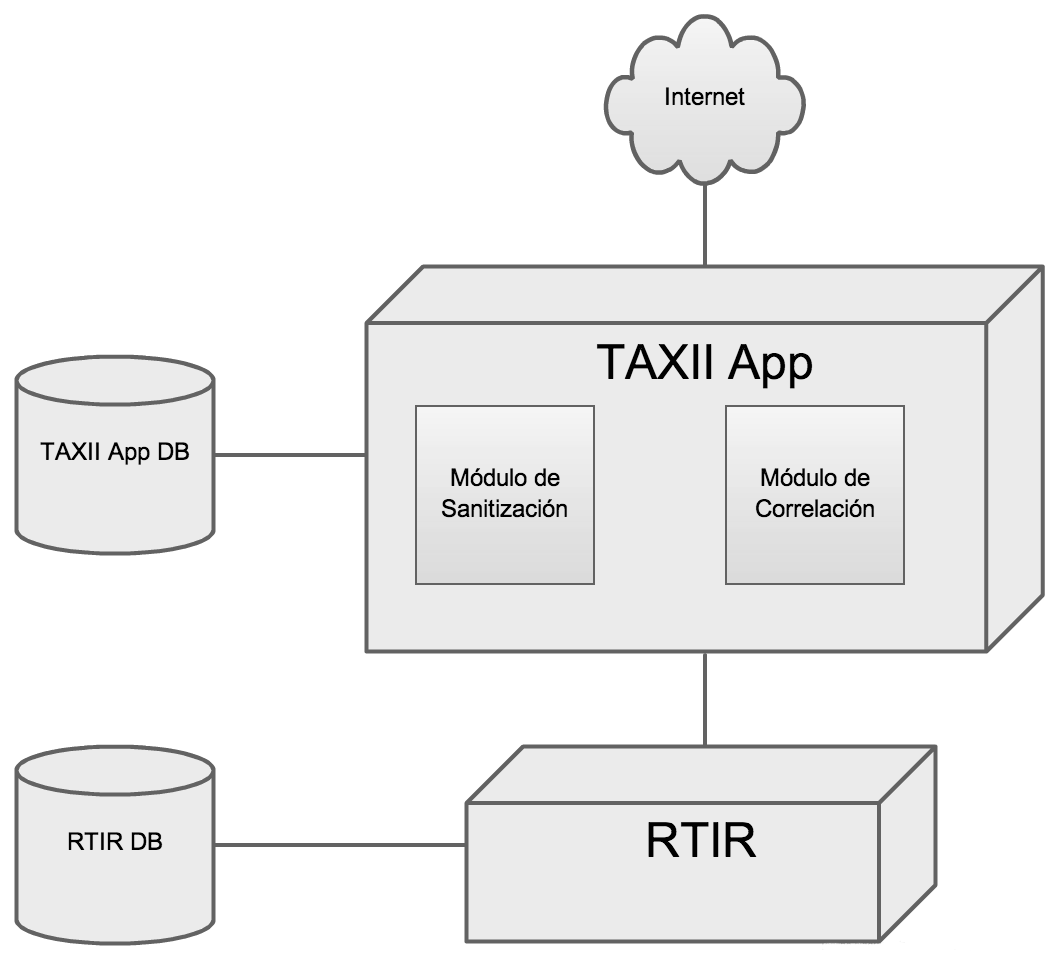
\includegraphics[width=1.9673in,height=1.7811in]{Analisis22-img/Analisis22-img016.png}
	\caption{Diagrama de Bloques del sistema}
	\label{fig.diagramabloques}
\end{figure}



\bigskip

{\selectlanguage{spanish}
	Con las herramientas mencionadas anteriormente podemos ver un diagrama de bloques como el de la figura \ref{fig.diagramabloques}. En la figura
	se puede ver que se cuenta con una instalación de la herramienta RTIR que será la encargada de la gestión de incidentes
	y por medio de la cual se dará de alta la información en el sistema. Además en el bloque ``TAXII App'' realiza el
	intercambio de información con otras organizaciones por medio de TAXII y representa la información utilizando STIX.
	Además dicho bloque es el encargado de realizar la sanitización y correlación de información.}


\bigskip


\bigskip

\section{Actores y Casos de Uso}
\subsection{Actores}

\bigskip

\begin{flushleft}
	\tablefirsthead{}
	\tablehead{}
	\tabletail{}
	\tablelasttail{}
	\begin{supertabular}{m{0.8608598in}m{4.89486in}}
		{\selectlanguage{spanish} Actor} &
		{\selectlanguage{spanish} Analista}\\\hline
		\multicolumn{1}{m{0.8608598in}|}{{\selectlanguage{spanish} Descripción}} &
		\multicolumn{1}{m{4.89486in}|}{{\selectlanguage{spanish} Este actor tiene la posibilidad de ingresar nueva
				información en el sistema. Dicha información puede ser intercambiada con otro sistema. Con la información que se ha
				intercambiado el actor puede realizar un análisis de ella y hacer un manejo de los casos creados en el RTIR.}}\\
	\end{supertabular}
\end{flushleft}

\bigskip


\bigskip

\begin{flushleft}
	\tablefirsthead{}
	\tablehead{}
	\tabletail{}
	\tablelasttail{}
	\begin{supertabular}{m{0.8816598in}m{4.8740597in}}
		{\selectlanguage{spanish} Actor} &
		{\selectlanguage{spanish} Cliente TAXII}\\\hline
		\multicolumn{1}{m{0.8816598in}|}{{\selectlanguage{spanish} Descripción}} &
		\multicolumn{1}{m{4.8740597in}|}{{\selectlanguage{spanish} Este actor es el que interactúa con el sistema
				para intercambiar datos por medio del protocolo TAXII. El sistema tiene que dar soporte para dicho protocolo para que
				el intercambio sea exitoso.}}\\
	\end{supertabular}
\end{flushleft}

\bigskip

\subsection{Casos de uso y diagramas de secuencia}

\bigskip

\subsubsection{ABM de políticas de sanitización}
\begin{flushleft}
	\tablefirsthead{}
	\tablehead{}
	\tabletail{}
	\tablelasttail{}
	\begin{supertabular}{m{1.0573599in}|m{4.82056in}|}
		\multicolumn{1}{m{1.0573599in}}{{\selectlanguage{spanish} Nombre}} &
		\multicolumn{1}{m{4.82056in}}{{\selectlanguage{spanish} ABM de políticas de sanitización}}\\\hline
		{\selectlanguage{spanish} Actor} &
		{\selectlanguage{spanish} Analista}\\
		{\selectlanguage{spanish} Descripción} &
		{\selectlanguage{spanish} Estos casos de uso comienzan cuando el analista desea realizar el alta, baja o
			modificación de las políticas de sanitización. Por medio de estas se filtra la información que se desea intercambiar
			con otras organizaciones.}\\\hhline{~-}
	\end{supertabular}
\end{flushleft}

\bigskip


\begin{figure}[ht!]
	\centering
	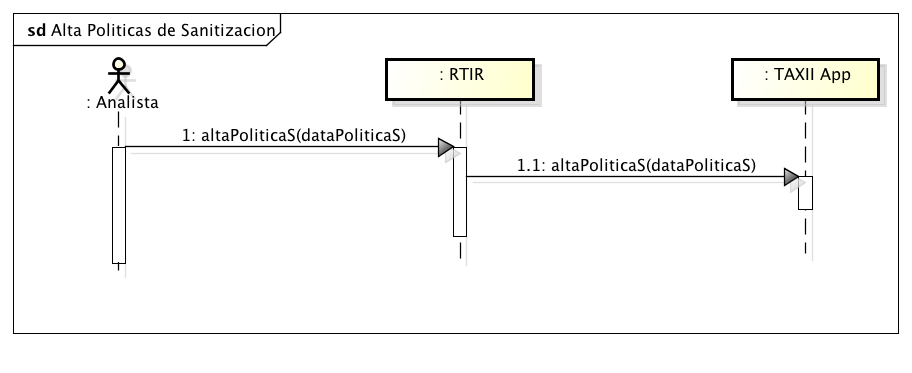
\includegraphics[width=5.7638in,height=2.3575in]{Analisis22-img/Analisis22-img017.png} 
	\caption{Caso de Uso alta políticas de sanitización}
	\label{fig.altasanitizacion}
\end{figure}
{\selectlanguage{spanish}
	\bigskip
	En la figura \ref{fig.altasanitizacion} se especifica el caso de uso, en este un analista ingresa a RTIR y da de alta en el sistema una política
	de sanitización. Dicha política es utilizada para realizar la sanitización de la información intercambiada por la
	organización. Las políticas son registradas en TAXII App.}
\begin{figure}[ht!]
	\centering
	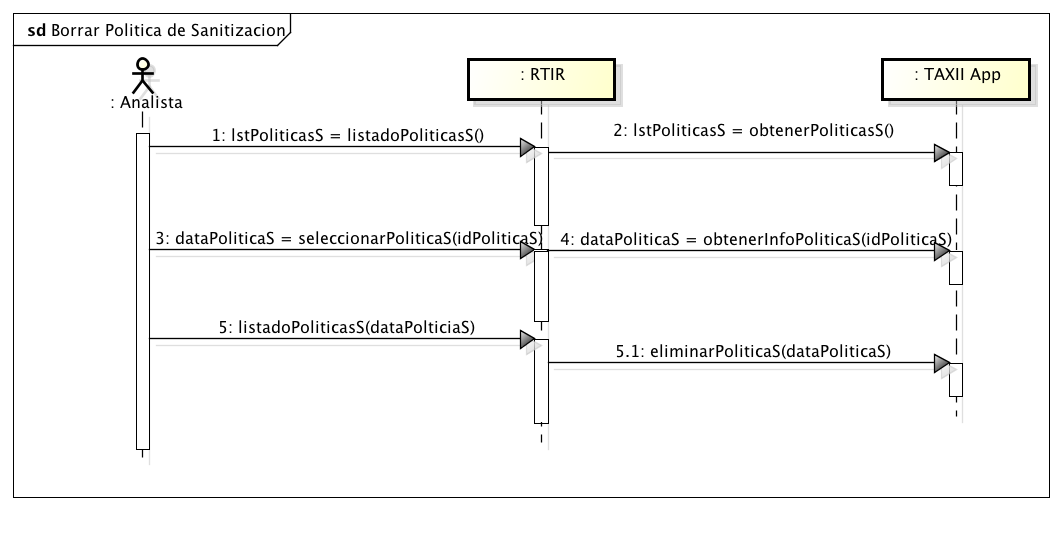
\includegraphics[width=5.7638in,height=2.9146in]{Analisis22-img/Analisis22-img018.png} 
	\caption{Caso de uso borrado políticas de sanitización}
	\label{fig.borradosanitizacion}
\end{figure}

\bigskip

{\selectlanguage{spanish}
	En la figura \ref{fig.borradosanitizacion} se especifica el caso de uso de borrado de políticas de sanitización, en este un analista ingresa a RTIR
	y lista todas las políticas disponibles en el sistema. Luego selecciona la política que desea dar de baja para luego
	borrarla.}


\newpage
\begin{figure}[ht!]
	\centering
	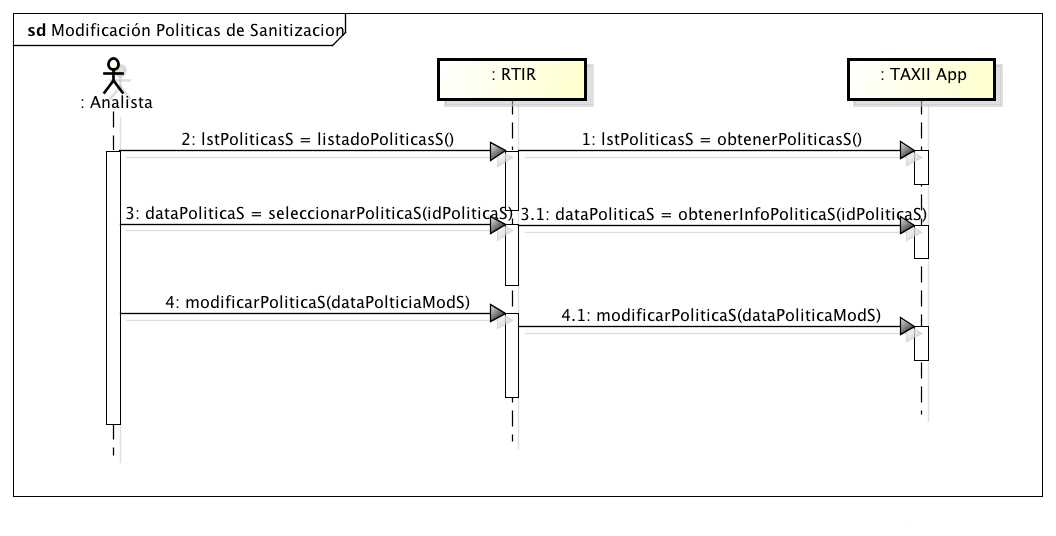
\includegraphics[width=5.7638in,height=2.9256in]{Analisis22-img/Analisis22-img019.png} 
	\caption{Caso de uso modificación de políticas de sanitización}
	\label{fig.modificacionsanitizacion}
\end{figure}
\bigskip
{\selectlanguage{spanish}
	En la figura \ref{fig.modificacionsanitizacion} se especifica el caso de uso de modificación de políticas de sanitización, en este un analista ingresa a
	RTIR y lista todas las políticas disponibles en el sistema. Luego selecciona la política que desea modificar.}
\newpage
\subsubsection[ABM de Políticas de Correlación]{\foreignlanguage{spanish}{ABM de Políticas de Correlación}}
\begin{flushleft}
	\tablefirsthead{}
	\tablehead{}
	\tabletail{}
	\tablelasttail{}
	\begin{supertabular}{m{1.0573599in}|m{4.82056in}|}
		\multicolumn{1}{m{1.0573599in}}{{\selectlanguage{spanish} Nombre}} &
		\multicolumn{1}{m{4.82056in}}{{\selectlanguage{spanish} ABM de políticas de correlación}}\\\hline
		{\selectlanguage{spanish} Actor} &
		{\selectlanguage{spanish} Analista}\\
		{\selectlanguage{spanish} Descripción} &
		{\selectlanguage{spanish} Estos casos de uso comienzan cuando el analista desea realizar el alta, baja o
			modificación de las políticas de correlación. Por medio de estas se agrupa la información según los datos existentes en
			el sistema.}\\\hhline{~-}
	\end{supertabular}
\end{flushleft}

\bigskip
\begin{figure}[ht!]
	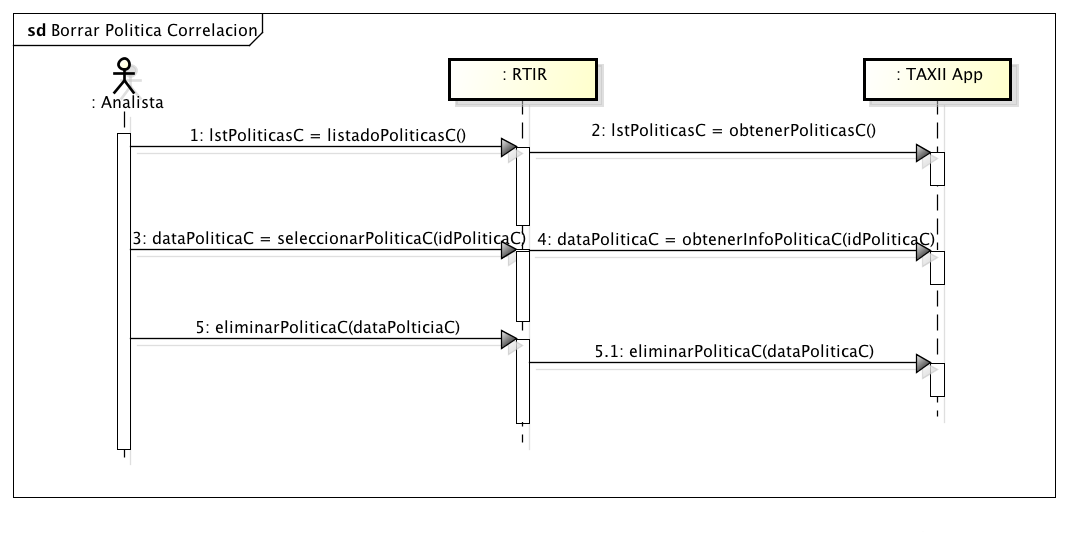
\includegraphics[width=5.7634in,height=2.898in]{Analisis22-img/Analisis22-img020.png}
	\caption{Caso de uso borrado políticas de correlación} 
	\label{fig.borradocorrelacion}
\end{figure}
{\selectlanguage{spanish}
	En la figura \ref{fig.borradocorrelacion} se especifica el caso de uso de borrado de políticas de correlación, en este un analista ingresa a RTIR y
	lista todas las políticas disponibles en el sistema. Luego selecciona la política que desea dar de baja para luego
	borrarla.}


\bigskip


\bigskip
\begin{figure}[ht!]
	\centering
	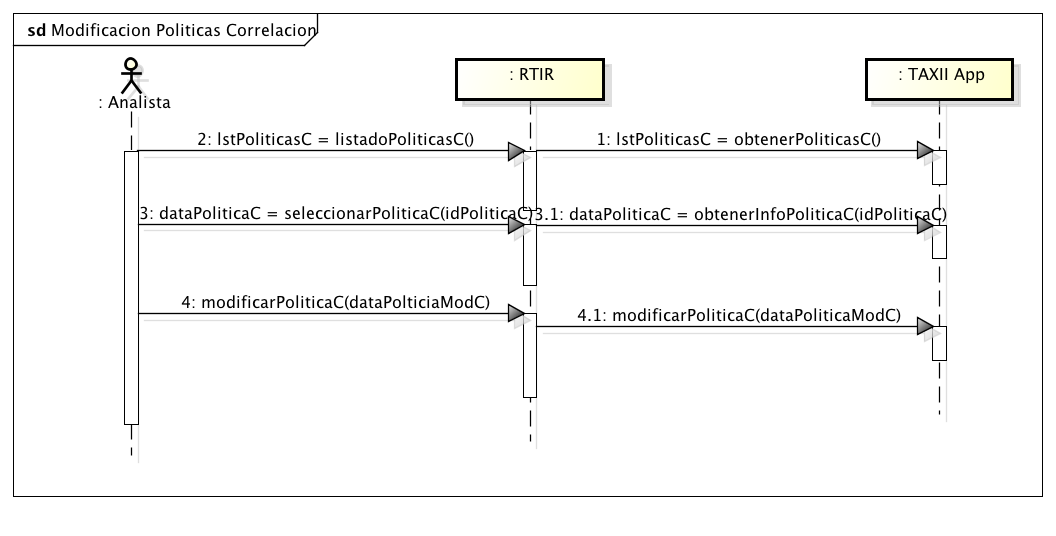
\includegraphics[width=5.7638in,height=2.9256in]{Analisis22-img/Analisis22-img021.png} 
	\caption{Caso de uso modificación políticas de correlación}
	\label{fig.modificacioncorrelacion}
\end{figure}
{\selectlanguage{spanish}
	En la figura \ref{fig.modificacioncorrelacion} se especifica el caso de uso de modificación de políticas de correlación, en este un analista ingresa a
	RTIR y lista todas las políticas disponibles en el sistema. Luego selecciona la política que desea modificar.}


\bigskip
\begin{figure}[ht!]
	\centering
	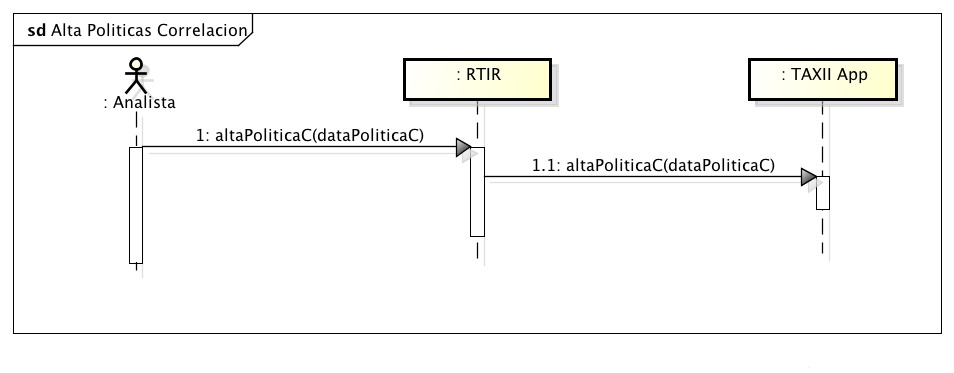
\includegraphics[width=5.7638in,height=2.2535in]{Analisis22-img/Analisis22-img022.png} 
	\caption{Caso de uso alta políticas de correlación}
	\label{fig.altacorrelacion}
\end{figure}
{\selectlanguage{spanish}
	En la figura \ref{fig.altacorrelacion} se especifica el caso de uso de alta de políticas de correlación, en este un analista ingresa a RTIR y
	da de alta en el sistema una política de correlación. Dicha política es utilizada para realizar la correlación de la
	información presente en el sistema. Las políticas son registradas en TAXII App.}


\newpage

\subsubsection{ABM de Servicios TAXII}

\bigskip

\begin{flushleft}
	\tablefirsthead{}
	\tablehead{}
	\tabletail{}
	\tablelasttail{}
	\begin{supertabular}{m{1.0573599in}|m{4.82056in}|}
		\multicolumn{1}{m{1.0573599in}}{{\selectlanguage{spanish} Nombre}} &
		\multicolumn{1}{m{4.82056in}}{{\selectlanguage{spanish} ABM de servicios TAXII}}\\\hline
		{\selectlanguage{spanish} Actor} &
		{\selectlanguage{spanish} Analista}\\
		{\selectlanguage{spanish} Descripción} &
		{\selectlanguage{spanish} Estos casos de uso comienzan cuando el analista desea realizar el alta, baja o
			modificación de servicio TAXII de otras organizaciones en el sistema. Estos serán utilizados para lograr el intercambio
			de información.}\\\hhline{~-}
	\end{supertabular}
\end{flushleft}

\bigskip

\begin{figure}[ht!]
	\centering
	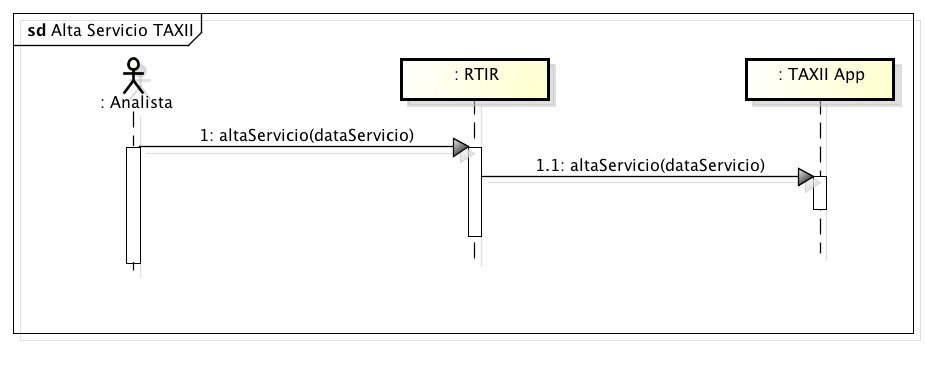
\includegraphics[width=5.7638in,height=2.3217in]{Analisis22-img/Analisis22-img023.png} 
	\caption{Caso de uso alta servicio TAXII}
	\label{fig.altaserviciotaxii}
\end{figure}
{\selectlanguage{spanish}
	En la figura \ref{fig.altaserviciotaxii} se especifica el caso de uso de alta de servicios TAXII, en este un analista ingresa a RTIR y da de alta
	en el sistema un servicio TAXII. Por medio de dicho servicio TAXII se realizara el intercambio con otra organización.}


\bigskip
\begin{figure}[ht!]
	\centering
	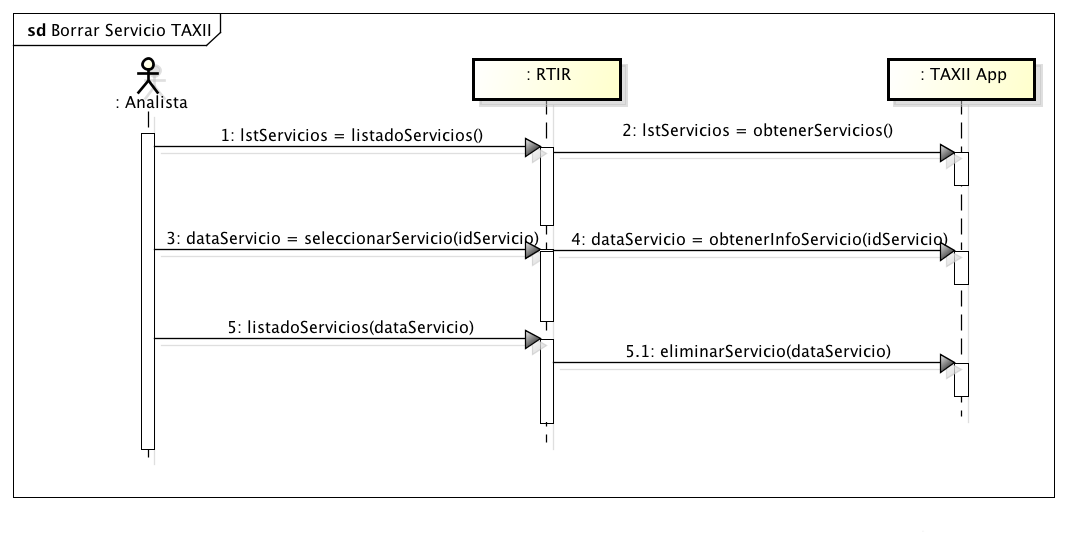
\includegraphics[width=5.7634in,height=2.898in]{Analisis22-img/Analisis22-img024.png} 
	\caption{Caso de uso borrar	servicio TAXII}
	\label{fig.borradoserviciotaxii}
\end{figure}
{\selectlanguage{spanish}
	En la figura \ref{fig.borradoserviciotaxii} se especifica el caso de uso de borrado de servicios TAXII, en este un analista ingresa a RTIR y lista
	todas las servicios disponibles en el sistema. Luego selecciona el que desea dar de baja.}
\newpage
\begin{figure}
	\centering
	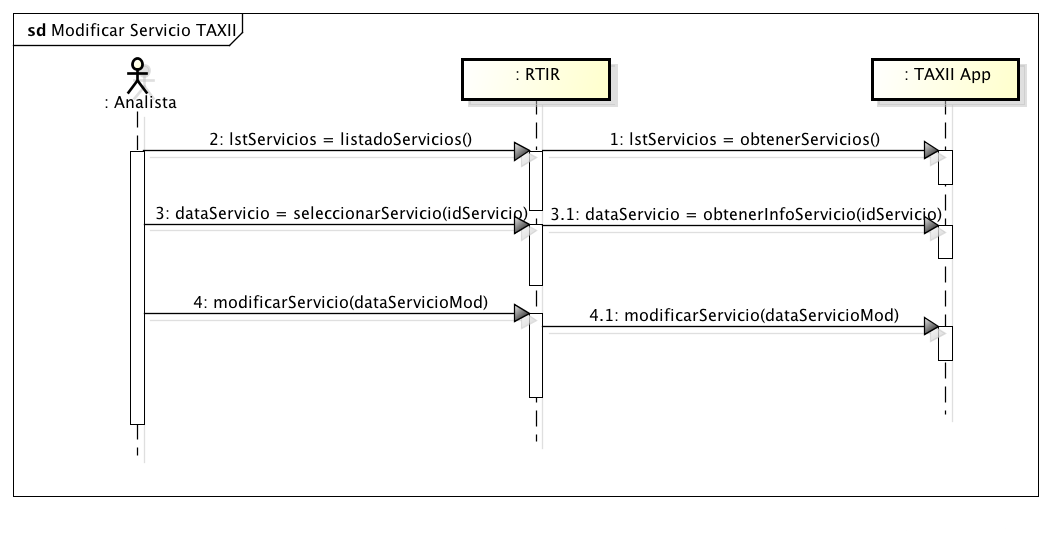
\includegraphics[width=5.7638in,height=2.9366in]{Analisis22-img/Analisis22-img025.png} 
	\caption{Caso de uso modificar servicio TAXII}
	\label{fig.modificarserviciotaxii}
\end{figure}

{\selectlanguage{spanish}
	En la figura \ref{fig.modificarserviciotaxii} se especifica el caso de uso de modificación de servicios TAXII, en este un analista ingresa a RTIR y
	lista todos los servicios disponibles. Luego selecciona el que será dado de baja.}
\newpage
\subsubsection{Alta de información RTIR}

\begin{flushleft}
	\tablefirsthead{}
	\tablehead{}
	\tabletail{}
	\tablelasttail{}
	\begin{supertabular}{m{0.8816598in}|m{4.8740597in}|}
		\multicolumn{1}{m{0.8816598in}}{{\selectlanguage{spanish} Nombre}} &
		\multicolumn{1}{m{4.8740597in}}{{\selectlanguage{spanish} Alta de información RTIR}}\\\hline
		{\selectlanguage{spanish} Actor} &
		{\selectlanguage{spanish} Analista}\\
		{\selectlanguage{spanish} Descripción} &
		{\selectlanguage{spanish} Este caso de uso comienza cuando el analista desea registrar nueva información en
			el sistema. Para ello debe ingresar la información deseada al sistema. Es deseado que se pueda dar de alta información
			referente a cyber observables como por ejemplo IPs, hash de archivos, descripciones de amenazas, etc. El manejo podría
			realizarse por medio de los incidentes de RTIR.}\\\hhline{~-}
	\end{supertabular}
\end{flushleft}

\begin{figure}
	\centering
	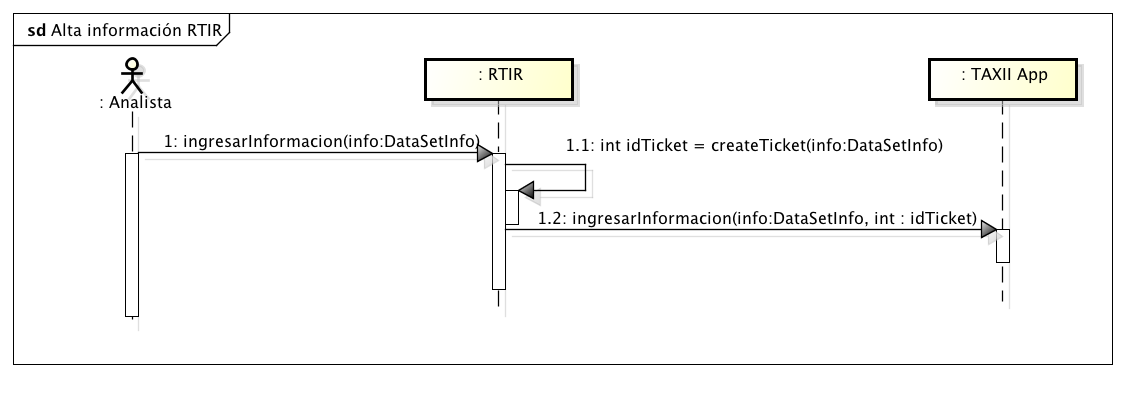
\includegraphics[width=5.7638in,height=2.0701in]{Analisis22-img/Analisis22-img026.png} 
	\caption{Caso de uso alta de información RTIR}
	\label{fig.altainfortir}
\end{figure}
{\selectlanguage{spanish}
	En la figura \ref{fig.altainfortir} se ve el caso de uso de alta de información en RTIR. En este un analista ingresa al sistema e ingresa
	nueva información en RTIR. En RTIR se crea un nuevo ticket y en TAXII App se da de alta la información representando y
	almacenándola de forma estructurada.}


\newpage
\subsubsection{Subscripción a TAXII Data Feed}
\begin{flushleft}
	\tablefirsthead{}
	\tablehead{}
	\tabletail{}
	\tablelasttail{}
	\begin{supertabular}{m{0.8816598in}|m{4.8740597in}|}
		\multicolumn{1}{m{0.8816598in}}{{\selectlanguage{spanish} Nombre}} &
		\multicolumn{1}{m{4.8740597in}}{{\selectlanguage{spanish} \foreignlanguage{spanish}{Subscripción a Taxii
					Data Feed}}}\\\hline
		{\selectlanguage{spanish} Actor} &
		{\selectlanguage{spanish} Analista}\\
		{\selectlanguage{spanish} Descripción} &
		{\selectlanguage{spanish} Con este caso de uso un analista selecciona un data feed en otro sistema al que
			quiere subscribirse. Esto se realiza por medio del Feed Managment Service de los sistemas.}\\\hhline{~-}
	\end{supertabular}
\end{flushleft}

\bigskip
\begin{figure}[ht!]
	\centering
	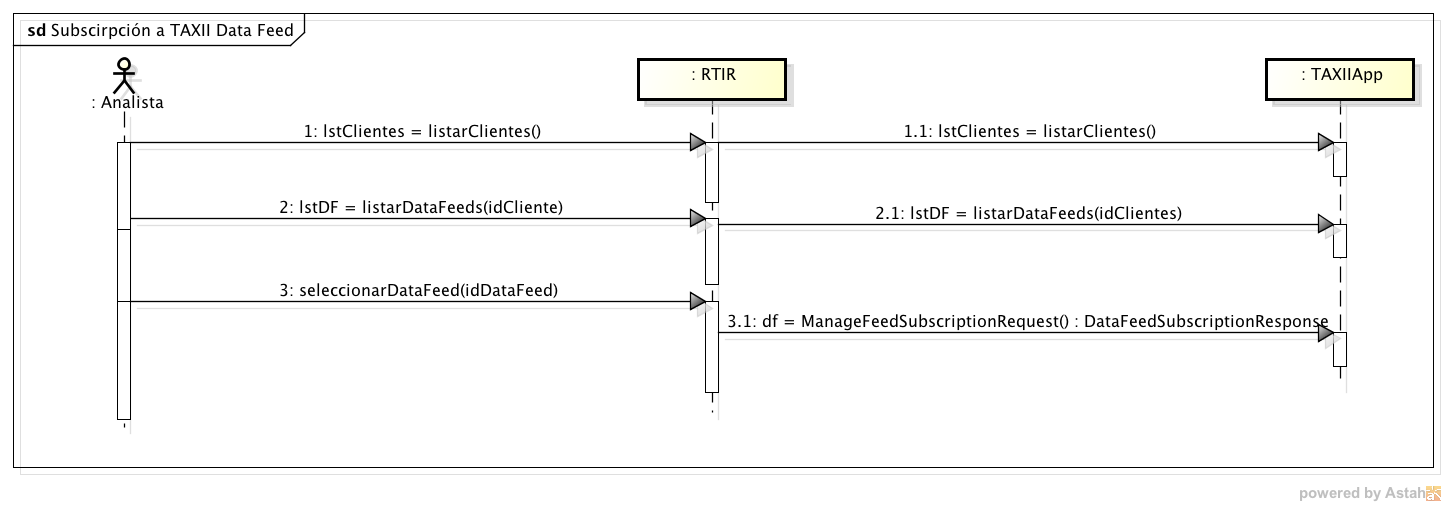
\includegraphics[width=5.4217in,height=1.8965in]{Analisis22-img/Analisis22-img027.png}
	\caption{Caso de uso subscripción a TAXII Data Feed}
	\label{fig.subscripciontaxiidatafeed}

\end{figure}

{\selectlanguage{spanish}
	En este caso de uso el analista desea subscribirse a uno de los TAXII data feed provistos por otra organización. Para
	ello obtiene un listado de los clientes TAXII con los que se relaciona para luego obtener un listado de los Data Feeds
	disponibles en ese cliente. Finalmente selecciona el TAXII data feed deseado. }

\newpage
\subsubsection{Recepción de información}
\begin{flushleft}
	\tablefirsthead{}
	\tablehead{}
	\tabletail{}
	\tablelasttail{}
	\begin{supertabular}{m{0.8816598in}|m{4.8740597in}|}
		\multicolumn{1}{m{0.8816598in}}{{\selectlanguage{spanish} Nombre}} &
		\multicolumn{1}{m{4.8740597in}}{{\selectlanguage{spanish} Recepción de información}}\\\hline
		{\selectlanguage{spanish} Actor} &
		{\selectlanguage{spanish} Cliente TAXII}\\
		{\selectlanguage{spanish} Descripción} &
		{\selectlanguage{spanish} Este caso de uso se da cuando un cliente TAXII desea enviarle información a
			nuestro sistema. El envío de información se realiza porque un analista se subscribió a un data feed en el cliente. La
			recepción de información se realiza por medio del Inbox Service de nuestro sistema.}\\\hhline{~-}
	\end{supertabular}
\end{flushleft}
\begin{figure}[ht!]
	\centering
	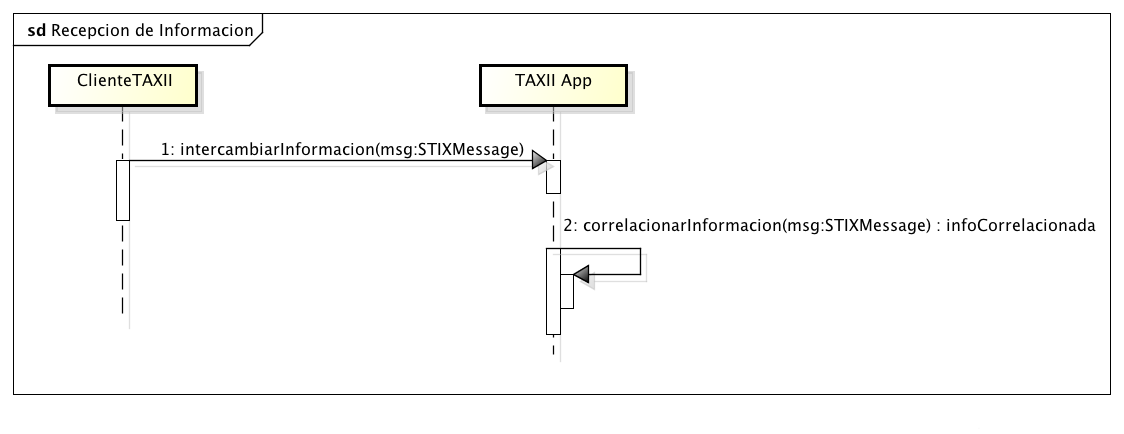
\includegraphics[width=5.7638in,height=2.2256in]{Analisis22-img/Analisis22-img028.png} 
	\caption{Caso de uso de recepción de información}
	\label{fig.recepcioninfo}
\end{figure}

{\selectlanguage{spanish}
	En este caso de uso un cliente TAXII en otra organización envía información a TAXII App. Luego la aplicación
	correlaciona la nueva información con la ya existente en el sistema.}
\newpage
\subsubsection{Envío de información}
\begin{flushleft}
	\tablefirsthead{}
	\tablehead{}
	\tabletail{}
	\tablelasttail{}
	\begin{supertabular}{m{0.8816598in}|m{4.8740597in}|}
		\multicolumn{1}{m{0.8816598in}}{{\selectlanguage{spanish} Nombre}} &
		\multicolumn{1}{m{4.8740597in}}{{\selectlanguage{spanish} Envío de información}}\\\hline
		{\selectlanguage{spanish} Actor} &
		{\selectlanguage{spanish} TAXII App}\\
		{\selectlanguage{spanish} Descripción} &
		{\selectlanguage{spanish} Este caso de uso se da cuando el sistema desea enviar información a otro cliente
			TAXII. El envío de información se realiza porque el cliente se subscribió al TAXII Data Feed del sistema. Esto se
			realiza por medio del Inbox Service del cliente. El intercambio es iniciado por el sistema.}\\\hhline{~-}
	\end{supertabular}
\end{flushleft}
\begin{figure}[ht!]
	\centering  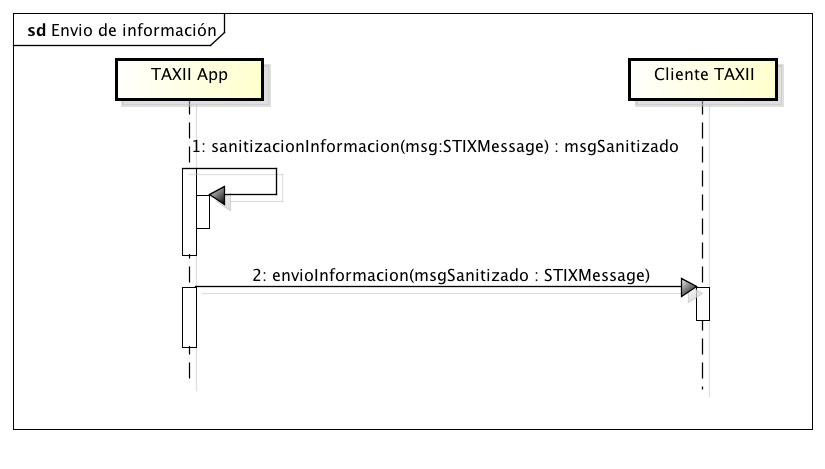
\includegraphics[width=5.7638in,height=3.2764in]{Analisis22-img/Analisis22-img029.png}
	\caption{Caso de uso de envío de información}
	\label{fig.enviodeinfo}
\end{figure}

{\selectlanguage{spanish}
	En este caso de uso TAXII App se comporta como el Actor y desea enviar nueva información a un cliente TAXII. Para ello
	lo primero que debe hacer es sanitizar la información. Luego envía la información representada en la forma de un
	mensaje STIX. Esto se ve en la figura \ref{fig.enviodeinfo}.}
\newpage
\subsubsection{Poll de información}
\begin{flushleft}
	\tablefirsthead{}
	\tablehead{}
	\tabletail{}
	\tablelasttail{}
	\begin{supertabular}{m{0.8816598in}|m{4.8740597in}|}
		\multicolumn{1}{m{0.8816598in}}{{\selectlanguage{spanish} Nombre}} &
		\multicolumn{1}{m{4.8740597in}}{{\selectlanguage{spanish} Poll de información}}\\\hline
		{\selectlanguage{spanish} Actor} &
		{\selectlanguage{spanish} TAXII App}\\
		{\selectlanguage{spanish} Descripción} &
		{\selectlanguage{spanish} Este caso de uso se da cuando un cliente desea recibir información de un
			productor TAXII, en este los intercambios son iniciados por el cliente que contacta al Poll Service del
			productor.}\\\hhline{~-}
	\end{supertabular}
\end{flushleft}

\bigskip
\begin{figure}
	\centering  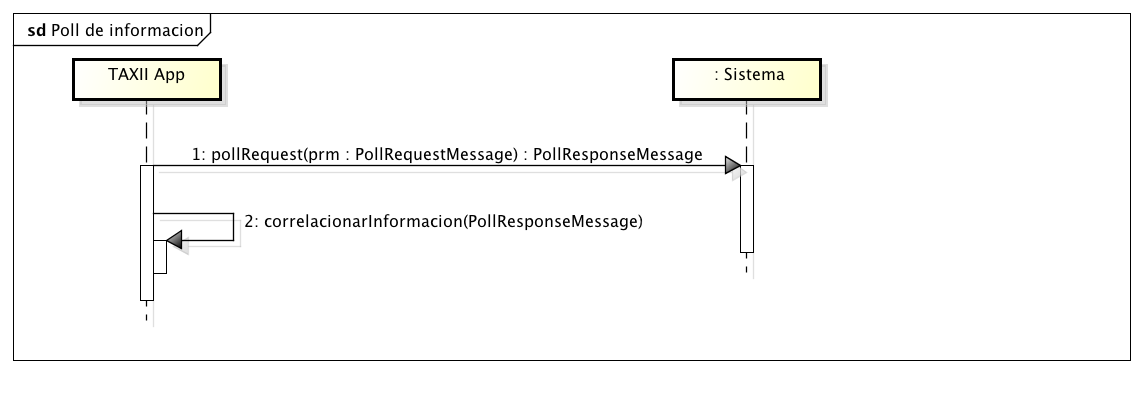
\includegraphics[width=5.7638in,height=2.0154in]{Analisis22-img/Analisis22-img030.png}
	\caption{Caso de uso de poll de
		información}
	\label{fig.pollinfo}
\end{figure}
{\selectlanguage{spanish}
	En la figura \ref{fig.pollinfo} se ve el caso de uso de poll de información. En este TAXII App realiza el pedido de información a otro
	cliente TAXII por medio de mensajes Poll Request. Cuando obtiene la información esta se correlaciona con los datos
	existentes en el sistema.}


\bigskip


\bigskip

{\selectlanguage{spanish}
	También se deben considerar los casos de uso provistos por RTIR para el seguimiento y manejo de los incidentes los
	cuales no serán especificados en este documento ya que se pueden encontrar en \foreignlanguage{spanish}{[RTIR]}. Dichos
	casos de uso permiten el manejo de \textit{tickets}, \textit{queues }y gestión de usuarios. }

{\selectlanguage{spanish}
	Con RTIR se especifica un \textit{workflow} para el trabajo con los \textit{tickets} en organizaciones de seguridad.
	Dicho \textit{workflow} comienza cuando se reporta un incidente, dicho reporte de incidente se asocia a un incidente o
	se crea uno nuevo. Los incidentes tratan de registrar toda la información necesaria para resolver el problema. De los
	incidentes se pueden iniciar investigaciones para trabajar con otras organizaciones. También se pueden crear
	\textit{blocks} para mantener un registro de las acciones realizadas para mitigar el incidente.}

%\newpage en otro lado
%\nocite{*}
%\bibliographystyle{plain} 
%\bibliography{bibliography}
